\documentclass[]{IEEEtran}
% some very useful LaTeX packages include:
%\usepackage{cite}      
\usepackage{graphicx}   
\usepackage{subfigure} 
\usepackage{url}       
\usepackage{amsmath}    
\usepackage{caption2}
% Your document starts here!
\begin{document}

% Define document title and author
	\title{Weekly Report}
	\author{Adviser: Prof. Yang Wen \\Student: Cheng Wensheng\\ Period: 2018.4.16-4.20
	}
	\markboth{Visual Information Processing Group}{}
	\maketitle

% Write abstract here
\begin{abstract}
	This week I mainly put my effort on revising CETC 54 technical report.
\end{abstract}

% Each section begins with a \section{title} command
\section{Work summary}
	% \PARstart{}{} creates a tall first letter for this first paragraph
	\PARstart{I}{n} work summary report, the first party raised following questions, and we revised them correspondingly. 
	\begin{itemize}
		\item About semantic annotation, they think we didn't state the annotation process clearly. Besides, since GAN didn't work well on our dataset, there is no need to introduce it in detail. So I delete contents about GAN, then fill semantic annotation part with Refine Net, which got the best result.
		\item About Content Based Image Retrieval(CBIR) process, they argue that we didn't explain this in detail, and we only presented CAMs. As for this, I add specific illustration about CBIR and similarity based image retrieval.
		\item Fig.~\ref{fig:mp} is CBIR flow chart. Fig.~\ref{fig:ss} is semantic segmentation results.
	\end{itemize}

% Main Part
\section{Technical summary}
	% LaTeX takes complete care of your document layout ...
	In technical summary report, they focus on CBIR and semantic annotation parts.
	\begin{itemize}
		\item About CBIR, they suggest we put more attention to the concrete procedure. Therefore, I add CBIR flow chart and detailed account based on our PowerPoint file.
		\item About semantic annotation, they claimed we just listed some methods without comparing them. In response to this, I add our experiment result table to this part, and compare them by P-R curve and mIoU. That should be enough.
		
	\end{itemize}
\newpage
\begin{figure}[!hbt]
%		 Center the figure.
		\vspace{2cm}
%		\hspace{50cm}
		\begin{center}
			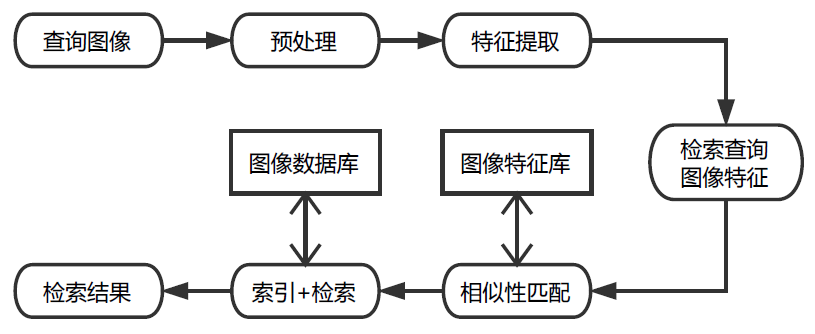
\includegraphics[width=\columnwidth]{flow}
				%		 Create a subtitle for the figure.
			\caption{CBIR flow chart}
			\label{fig:mp}
		    \hspace{0.5cm}
			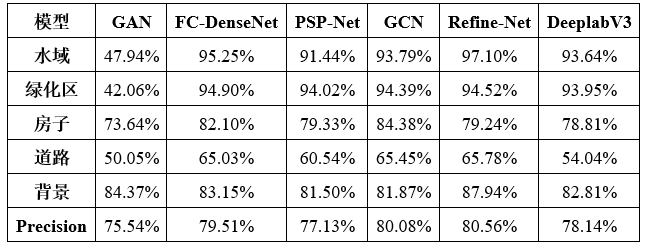
\includegraphics[width=\columnwidth]{result}
				%Create a subtitle for the figure.
			\caption{Semantic segmentation results}
			\label{fig:ss}
		\end{center}
	\end{figure}

% Now we need a bibliography:
%\begin{thebibliography}{5}
%
%	%Each item starts with a \bibitem{reference} command and the details thereafter.
%	\bibitem{HOP96} % Transaction paper
%	J.~Hagenauer, E.~Offer, and L.~Papke. Iterative decoding of binary block
%	and convolutional codes. {\em IEEE Trans. Inform. Theory},
%	vol.~42, no.~2, pp.~429–-445, Mar. 1996.
%
%	\bibitem{MJH06} % Conference paper
%	T.~Mayer, H.~Jenkac, and J.~Hagenauer. Turbo base-station cooperation for intercell interference cancellation. {\em IEEE Int. Conf. Commun. (ICC)}, Istanbul, Turkey, pp.~356--361, June 2006.
%
%	\bibitem{Proakis} % Book
%	J.~G.~Proakis. {\em Digital Communications}. McGraw-Hill Book Co.,
%	New York, USA, 3rd edition, 1995.
%
%	\bibitem{talk} % Web document
%	F.~R.~Kschischang. Giving a talk: Guidelines for the Preparation and Presentation of Technical Seminars.
%	\url{http://www.comm.toronto.edu/frank/guide/guide.pdf}.
%
%	\bibitem{5}
%	IEEE Transactions \LaTeX and Microsoft Word Style Files.
%	\url{http://www.ieee.org/web/publications/authors/transjnl/index.html}
%
%\end{thebibliography}

% Your document ends here!
\end{document}